Although mobile phones have many different devices on-chip that could be
potentially used as sources of randomness for a random number generator, most of
these devices have the potential for strong bias.  Additionally, because of the
operating environment, polling these devices with high frequency can cause
serious system performance and energy issues.  Therefore, it is necessary to not
only use devices that have high quality randomness, but to use those devices in
an intelligent manner so as to not overwhelm the computational and energy
resources of the device.

We propose the implementation of a Android process that polls data from the
accelerometer and gyroscope (when the entropy pool is running low), processes
input data to eliminate sources of bias, and feeds the data into the entropy
pool.  Fig.~\ref{proposed_solution_block} shows the architecture for our
application. Android built on Linux exposes standard interfaces to the hardware
sensors for data retrieval; additionally, Linux provides system calls to feed
random data into the entropy pool.  Our application will interact with both of
these interfaces.

%There are many types of post processing that can be implemented to increase the
%uniformity of the random numbers generated.  Hash algorithms like SHA-3
%\cite{keccak} can be used to eliminate bias.  Similarly, Barak et al. propose a
%technique whereby random numbers are pulled from several independent devices
%\cite{independent_devices}.  Two of these numbers are multiplied together and
%added to a third number to strengthen the randomness.  Barak et al. propose
%another technique where random numbers are multiplied by a Toeplitz matrix to
%approach a uniform distribution \cite{true_rng}.  These techniques will be
%implemented and compared for their effectiveness and computational complexity.
%
%Random numbers generated by our daemon will be compared to the stock
%Android/Linux random number generator (which includes an on-board hardware RNG
%that may not be present on all mobile devices).  These two sources will be
%compared on three dimensions: quality of random numbers generated, energy draw
%from using the random number generator, and computational resources used by
%random number generation.  The DIEHARD \cite{diehard} / NIST \cite{nist}
%benchmarks will be used to evaluate the quality of the random numbers
%generated; synthetic benchmarks will be written to evaluate the energy draw and
%computational complexity of the random number generators.

%just mention V. N. Whitening here?

%There are many types of post processing that can be implemented to increase the
%uniformity of the random numbers generated.  Hash algorithms like SHA-3
%\cite{keccak} can be used to eliminate bias.  Similarly, Barak et al. propose a
%technique whereby random numbers are pulled from several independent devices
%\cite{independent_devices}.  Two of these numbers are multiplied together and
%added to a third number to strengthen the randomness.  Barak et al. propose
%another technique where random numbers are multiplied by a Toeplitz matrix to
%approach a uniform distribution \cite{true_rng}.  These techniques will be
%implemented and compared for their effectiveness and computational complexity.

There are many types of post processing that can be implemented to increase the
uniformity of the random numbers generated. The post-processing proposed for the
scope of this paper is Von Neumann Whitening \cite{vn_whitening} and basic bit
filtering. 

\begin{figure}
	\centering
	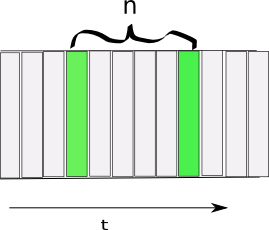
\includegraphics[width=0.25\textwidth]{vn_whitening.png}
	\caption{von Neumann whitening across several samples.}
	\label{fig:vnw}
\end{figure}

Von Neumann Whitening is a basic post processing procedure that takes two bits
at a time and processes them to give three possible outcomes. If the two bits
are the same, then they are simply discarded and there is no output. If the
sequence of bits is 0,1 then the output is 1 and conversely if the sequence of
bits is 1,0 then the output is 0. The rational behind this scheme is that it
will eliminate bias of the bits source towards a 1 or a 0. If the source is
biased towards either value with probability $p$, the probabilities for 1,0 and
0,1 are both equal to $p(1-p)$. With the same probability, they become a single
entropic bit. Unfortunately, this method only works to eliminate bias, but not
correlation between bits. The proposed solution attempts to reduce correlation
by using bits from samples taken $N$ samplings apart as can be seen in figure
\ref{fig:vnw} (in this case, $N = 1024$) and by using bit positions that are
offset from each other. 

The other method of improving the quality of the data that is pulled from the
sensors that is explored in this work is basic bit filtering. This is the simple
process of reading in all bits from the original source, and discarding those
that are suspected to be less random. Owing to the type of source that is being
polled, sensors, not all of the bits can be expected to be highly entropic or
even partially random. The data that can be retrieved from the Android sensor
API is returned as an IEEE 754 floating point number. As a result we can
immediately assume that both the sign bit and the exponent are unlikely to vary
much during normal use and are highly likely to be correlated between samplings.
Similarly, the most significant bits of the mantissa are intuitively more likely
to be correlated between samples than the least significant bit. The proposed
solution discards those bits that are suspected, through preimplementation
testing, of being of lesser quality randomness, though an ideal solution would
be able to sense the randomness of its incoming streams and filter accordingly
at runtime.
